\documentclass[10pt]{article}

\usepackage[margin=0.68in]{geometry}
\usepackage[T1]{fontenc}
\usepackage{lmodern}
\usepackage{amsmath,amssymb}
\usepackage{booktabs}
\usepackage{array}
\usepackage{tikz}
\usetikzlibrary{calc,positioning}
\usepackage{circuitikz}
\usepackage{listings}
\usepackage{verbatim}
\usepackage{xcolor}
\usepackage{fancyhdr}
\usepackage[hidelinks]{hyperref}

\definecolor{headc}{HTML}{1F3864}
\definecolor{gac}{HTML}{1565C0}
\definecolor{gad}{HTML}{2E7D32}
\definecolor{gbc}{HTML}{EF6C00}
\definecolor{gbd}{HTML}{6A1B9A}

\setlength{\parindent}{0pt}
\setlength{\parskip}{0.35em}
\pagestyle{fancy}
\fancyhf{}
\fancyhead[L]{\scriptsize EECE 7205 \textbar\ Stacks and Queues In-Class Work}
\fancyhead[R]{\scriptsize MyungJin Suh}
\fancyfoot[C]{\scriptsize\thepage}
\renewcommand{\headrulewidth}{0.3pt}
\hypersetup{pdftitle={EECE 7205 Stacks and Queues In-Class Work},pdfauthor={MyungJin Suh}}

\lstset{
  language=C++,
  basicstyle=\ttfamily\footnotesize,
  columns=fullflexible,
  keepspaces=true,
  breaklines=true,
  frame=single,
  framerule=0.3pt,
  rulecolor=\color{headc!40},
  xleftmargin=0.4em,
  framexleftmargin=0.4em
}

\ctikzset{logic ports=american}
\newcommand{\prob}[1]{%
  \par\vspace{6pt}{\large\bfseries\color{headc}#1}\par\vspace{1pt}%
  \noindent\textcolor{headc}{\rule{\linewidth}{0.6pt}}\par\vspace{2pt}}
\newcommand{\task}[1]{\par\vspace{2pt}\noindent\textbf{#1}\par\vspace{1pt}}

\begin{document}

\begin{center}
{\LARGE\bfseries\color{headc} Stacks and Queues}\\[0.25em]
{\large In-Class Work}\\[0.45em]
MyungJin Suh\\
EECE 7205
\end{center}

\prob{Q1 \quad Expression evaluation using stacks}

Two stacks, both with the top at the back of a vector. \texttt{values} holds integers. \texttt{ops} holds operators. The expression is a \texttt{vector<string>}. A token such as \texttt{-7} is one number, not a minus operator.

\texttt{isNumber} accepts an optional leading minus and then digits.
\texttt{precedence} is 1 for \texttt{+} and \texttt{-}, 2 for \texttt{*} and \texttt{/}, 3 for \textasciicircum.
An incoming operator pops the stack while the top has higher precedence, or equal precedence when the incoming operator is not \textasciicircum. That leaves \texttt{2 \textasciicircum\ 3 \textasciicircum\ 2} as \(2^{(3^{2})}\).
\texttt{apply} does the arithmetic. Division uses the C++ quotient, then subtracts 1 when the remainder is nonzero and the signs differ, which rounds toward \(-\infty\).
\texttt{evaluate} walks the tokens, then empties \texttt{ops}.

\lstinputlisting{expression.cpp}

\task{(b) and (c) \quad \(8 + 3 \times 2^{2} - 20/4\)}

Top is the right-hand end of each stack. A blank token line is a reduction caused by the next operator. \texttt{remaining} is the stack after the last token.

\verbatiminput{output.txt}

The value is 15.
\(2^{2} = 4\), then \(3 \times 4 = 12\), then \(8 + 12 = 20\).
The minus has lower precedence than \textasciicircum, \texttt{*}, and \texttt{+}, so those three run before \texttt{-} is pushed.
Then \(20 / 4 = 5\) and \(20 - 5 = 15\).

\task{(d) \quad Associativity and division}

\(2 \mathbin{\textasciicircum} 3 \mathbin{\textasciicircum} 2\): the second \textasciicircum\ does not pop the first, because the precedences are equal and \textasciicircum\ is right-associative. The stack is \texttt{[2 3 2]} over \texttt{[\textasciicircum\ \textasciicircum]}. The remaining steps are \(3^{2} = 9\), then \(2^{9} = 512\). Left associativity would have produced \((2^{3})^{2} = 64\).

\(-7 / 2\): C++ gives \(-3\). The remainder is \(-1\), and the signs differ, so the quotient becomes \(-4\). That is \(\lfloor -7/2 \rfloor\).

\prob{Q2 \quad Logic gate analysis}

\begin{center}
\begin{tabular}{lll}
\toprule
Signal & Gate & Inputs \\
\midrule
\(N_1\) & NOT & \(C\) \\
\(N_2\) & NOT & \(D\) \\
\(P\) & OR & \(B,\ N_1\) \\
\(Q\) & AND & \(A,\ P\) \\
\(R\) & OR & \(C,\ N_2\) \\
\(S\) & AND & \(B,\ R\) \\
\(T\) & AND & \(A,\ D\) \\
\(Z\) & OR & \(Q,\ S,\ T\) \\
\bottomrule
\end{tabular}
\end{center}

\task{(a) \quad Circuit}

\begin{center}
\begin{circuitikz}[thick, font=\small]
  \node[and port] (q) at (10.0,8.0) {};
  \node[or port] (p) at (6.2,6.3) {};
  \node[not port] (n1) at (3.5,4.9) {};
  \node[and port] (s) at (10.0,3.5) {};
  \node[or port] (r) at (6.2,2.0) {};
  \node[not port] (n2) at (3.5,0.5) {};
  \node[and port] (t) at (10.0,-1.2) {};
  \node[or port, number inputs=3] (z) at (13.4,3.5) {};

  \draw (0,0 |- q.in 1) node[left] {$A$} -- (q.in 1);
  \draw (0.55,0 |- q.in 1) node[circ] {} coordinate (As)
        -- (0.55,0 |- t.in 1) -- (t.in 1);

  \draw (0,0 |- p.in 1) node[left] {$B$} -- (p.in 1);
  \draw (1.25,0 |- p.in 1) node[circ] {} coordinate (Bs)
        -- (1.25,0 |- s.in 1) -- (s.in 1);

  \draw (0,0 |- n1.in 1) node[left] {$C$} -- (n1.in 1);
  \draw (1.95,0 |- n1.in 1) node[circ] {} coordinate (Cs)
        -- (1.95,0 |- r.in 1) -- (r.in 1);

  \draw (0,0 |- n2.in 1) node[left] {$D$} -- (n2.in 1);
  \draw (2.65,0 |- n2.in 1) node[circ] {} coordinate (Ds)
        -- (2.65,0 |- t.in 2) -- (t.in 2);

  \draw (n1.out) -- ++(0.55,0) node[above,midway] {$N_1$} coordinate (n1o);
  \draw (n1o) |- (p.in 2);
  \draw (p.out) -- ++(0.55,0) node[above,midway] {$P$} coordinate (po);
  \draw (po) |- (q.in 2);

  \draw (n2.out) -- ++(0.55,0) node[above,midway] {$N_2$} coordinate (n2o);
  \draw (n2o) |- (r.in 2);
  \draw (r.out) -- ++(0.55,0) node[above,midway] {$R$} coordinate (ro);
  \draw (ro) |- (s.in 2);

  \draw (q.out) -- ++(1.15,0) node[above,pos=0.35] {$Q$} coordinate (qo);
  \draw (qo) |- (z.in 1);
  \draw (s.out) -- (z.in 2) node[above,midway] {$S$};
  \draw (t.out) -- ++(1.55,0) node[above,pos=0.25] {$T$} coordinate (to);
  \draw (to) |- (z.in 3);
  \draw (z.out) -- ++(0.55,0) node[right] {$Z$};
\end{circuitikz}
\end{center}

\task{(b) \quad Boolean expression}

\begin{align*}
N_1 &= C' & N_2 &= D' \\
P &= B + N_1 = B + C' &
Q &= AP = A(B + C') = AB + AC' \\
R &= C + N_2 = C + D' &
S &= BR = B(C + D') = BC + BD' \\
T &= AD \\
Z &= Q + S + T = AB + AC' + BC + BD' + AD
\end{align*}

\task{(c) \quad Truth table}

Each intermediate column is the gate in (b). \(Z = Q + S + T\).

\begin{center}
\small
\begin{tabular}{cccc ccccccc c}
\toprule
\(A\) & \(B\) & \(C\) & \(D\) & \(N_1\) & \(N_2\) & \(P\) & \(Q\) & \(R\) & \(S\) & \(T\) & \(Z\) \\
\midrule
0 & 0 & 0 & 0 & 1 & 1 & 1 & 0 & 1 & 0 & 0 & 0 \\
0 & 0 & 0 & 1 & 1 & 0 & 1 & 0 & 0 & 0 & 0 & 0 \\
0 & 0 & 1 & 0 & 0 & 1 & 0 & 0 & 1 & 0 & 0 & 0 \\
0 & 0 & 1 & 1 & 0 & 0 & 0 & 0 & 1 & 0 & 0 & 0 \\
\addlinespace
0 & 1 & 0 & 0 & 1 & 1 & 1 & 0 & 1 & 1 & 0 & 1 \\
0 & 1 & 0 & 1 & 1 & 0 & 1 & 0 & 0 & 0 & 0 & 0 \\
0 & 1 & 1 & 0 & 0 & 1 & 1 & 0 & 1 & 1 & 0 & 1 \\
0 & 1 & 1 & 1 & 0 & 0 & 1 & 0 & 1 & 1 & 0 & 1 \\
\addlinespace
1 & 0 & 0 & 0 & 1 & 1 & 1 & 1 & 1 & 0 & 0 & 1 \\
1 & 0 & 0 & 1 & 1 & 0 & 1 & 1 & 0 & 0 & 1 & 1 \\
1 & 0 & 1 & 0 & 0 & 1 & 0 & 0 & 1 & 0 & 0 & 0 \\
1 & 0 & 1 & 1 & 0 & 0 & 0 & 0 & 1 & 0 & 1 & 1 \\
\addlinespace
1 & 1 & 0 & 0 & 1 & 1 & 1 & 1 & 1 & 1 & 0 & 1 \\
1 & 1 & 0 & 1 & 1 & 0 & 1 & 1 & 0 & 0 & 1 & 1 \\
1 & 1 & 1 & 0 & 0 & 1 & 1 & 1 & 1 & 1 & 0 & 1 \\
1 & 1 & 1 & 1 & 0 & 0 & 1 & 1 & 1 & 1 & 1 & 1 \\
\bottomrule
\end{tabular}
\end{center}

\task{(d) \quad Karnaugh map}

Rows are \(AB\) and columns are \(CD\), both in Gray code. The four quads are \(AC'\), \(AD\), \(BC\), and \(BD'\). \(BD'\) uses the two outside columns.

\begin{center}
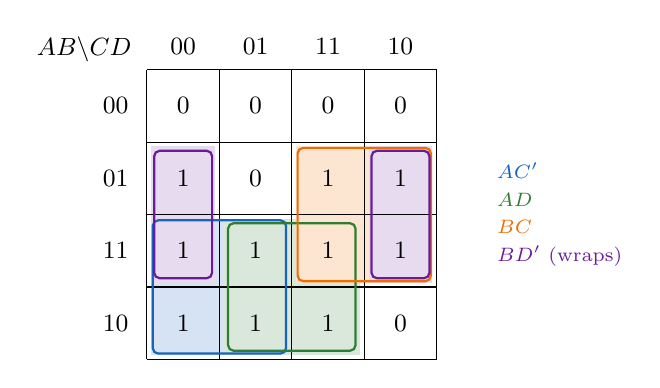
\begin{tikzpicture}[scale=0.92, every node/.style={font=\small}]
  \fill[gac!18] (0.06,0.06) rectangle (1.94,1.94);
  \fill[gad!18] (1.06,0.06) rectangle (2.94,1.94);
  \fill[gbc!18] (2.06,1.06) rectangle (3.94,2.94);
  \fill[gbd!16] (0.06,1.06) rectangle (0.94,2.94);
  \fill[gbd!16] (3.06,1.06) rectangle (3.94,2.94);

  \draw (0,0) grid (4,4);
  \node[anchor=east] at (-0.08,4.28) {\(AB \backslash CD\)};
  \foreach \x/\t in {0.5/00, 1.5/01, 2.5/11, 3.5/10}
    \node at (\x,4.32) {\t};
  \foreach \y/\t in {3.5/00, 2.5/01, 1.5/11, 0.5/10}
    \node[anchor=east] at (-0.12,\y) {\t};

  \node at (0.5,3.5) {0}; \node at (1.5,3.5) {0};
  \node at (2.5,3.5) {0}; \node at (3.5,3.5) {0};
  \node at (0.5,2.5) {1}; \node at (1.5,2.5) {0};
  \node at (2.5,2.5) {1}; \node at (3.5,2.5) {1};
  \node at (0.5,1.5) {1}; \node at (1.5,1.5) {1};
  \node at (2.5,1.5) {1}; \node at (3.5,1.5) {1};
  \node at (0.5,0.5) {1}; \node at (1.5,0.5) {1};
  \node at (2.5,0.5) {1}; \node at (3.5,0.5) {0};

  \draw[gac, thick, rounded corners=2pt] (0.08,0.08) rectangle (1.92,1.92);
  \draw[gad, thick, rounded corners=2pt] (1.12,0.12) rectangle (2.88,1.88);
  \draw[gbc, thick, rounded corners=2pt] (2.08,1.08) rectangle (3.92,2.92);
  \draw[gbd, thick, rounded corners=2pt] (0.10,1.12) rectangle (0.90,2.88);
  \draw[gbd, thick, rounded corners=2pt] (3.10,1.12) rectangle (3.90,2.88);

  \node[anchor=west, font=\scriptsize, align=left] at (4.7,2.0)
    {\textcolor{gac}{\(AC'\)}\\[0.25em]
     \textcolor{gad}{\(AD\)}\\[0.25em]
     \textcolor{gbc}{\(BC\)}\\[0.25em]
     \textcolor{gbd}{\(BD'\) (wraps)}};
\end{tikzpicture}
\end{center}

\(AB\) is already covered, so it drops out of the sum:
\begin{align*}
AB &= ABC + ABC' \\
&= ABCD + ABCD' + ABC'D + ABC'D' .
\end{align*}
\(ABCD\) and \(ABCD'\) are in \(BC\), \(ABC'D\) is in \(AD\), and \(ABC'D'\) is in \(BD'\). All four are also in \(AC'\) except the two terms that contain \(C\). Either way,
\[
Z = AC' + AD + BC + BD' .
\]
Each product is a quad, and each owns a 1 that the other three miss: \(AC'\) has \(m_8 = 1000\), \(AD\) has \(m_{11} = 1011\), \(BC\) has \(m_7 = 0111\), and \(BD'\) has \(m_4 = 0100\). Four products, eight literals. This is the minimum sum of products. Factored,
\[
Z = A(C' + D) + B(C + D') .
\]

\task{(e) \quad NAND only}

Seven 2-input NAND gates. A complement is a NAND with the inputs tied. The inner sums are NAND by De Morgan, and the outer sum is the NAND of the two inverted products.

\begin{align*}
C' &= (CC)' & D' &= (DD)' \\
C' + D &= (C \cdot D')' & C + D' &= (C' \cdot D)' \\
\big(A(C' + D)\big)' &= \big(A \cdot (C' + D)\big)' \\
\big(B(C + D')\big)' &= \big(B \cdot (C + D')\big)' \\
Z &= \Big(\big(A(C' + D)\big)' \cdot \big(B(C + D')\big)'\Big)'
\end{align*}

\begin{center}
\begin{circuitikz}[thick, font=\scriptsize]
  \node[nand port] (g1) at (3.3,4.2) {};
  \node[nand port] (g2) at (3.3,1.0) {};
  \node[nand port] (g3) at (7.0,5.5) {};
  \node[nand port] (g4) at (7.0,2.2) {};
  \node[nand port] (g5) at (10.6,6.2) {};
  \node[nand port] (g6) at (10.6,1.5) {};
  \node[nand port] (g7) at (13.6,3.8) {};

  \draw (g1.in 1) -- ++(-0.5,0) coordinate (cHi);
  \draw (g1.in 2) -- ++(-0.5,0) coordinate (cLo);
  \draw (cHi) -- (cLo);
  \coordinate (cMid) at ($(cHi)!0.5!(cLo)$);
  \draw (cMid) -- ++(-0.55,0) coordinate (cTap) -- ++(-0.9,0) node[left,font=\small] {$C$};
  \node[circ] at (cTap) {};

  \draw[red] (g2.in 1) -- ++(-0.5,0) coordinate (dHi);
  \draw[red] (g2.in 2) -- ++(-0.5,0) coordinate (dLo);
  \draw[red] (dHi) -- (dLo);
  \coordinate (dMid) at ($(dHi)!0.5!(dLo)$);
  \draw[red] (dMid) -- ++(-0.55,0) coordinate (dTap) -- ++(-0.9,0) node[left,font=\small,black] {$D$};
  \node[circ,red] at (dTap) {};

  \draw (g1.out) -- ++(0.7,0) node[above=2pt] {$C'$} coordinate (cbar);
  \draw[red] (g2.out) -- ++(1.35,0) node[above=2pt,black] {$D'$} coordinate (dbar);

  \draw (cTap) -- (cTap |- g3.in 1) -- (g3.in 1);
  \draw[red] (dbar) -- (dbar |- g3.in 2) -- (g3.in 2);
  \draw (g3.out) -- ++(0.85,0) node[above=7pt,pos=0.15] {$C'+D$} coordinate (g3o);
  \draw[red] (g3o) -- (g3o |- g5.in 2) -- (g5.in 2);

  \draw (cbar) -- (cbar |- g4.in 1) -- (g4.in 1);
  \draw (dTap) -- (dTap |- g4.in 2) -- (g4.in 2);
  \draw (g4.out) -- ++(0.85,0) node[above=7pt,pos=0.15] {$C+D'$} coordinate (g4o);
  \draw (g4o) -- (g4o |- g6.in 2) -- (g6.in 2);

  \draw (g5.in 1) -- ++(-0.8,0) node[left,font=\small] {$A$};
  \draw[red] (g5.out) -- ++(0.85,0) coordinate (g5o);
  \draw (g6.in 1) -- ++(-0.8,0) node[left,font=\small] {$B$};
  \draw (g6.out) -- ++(1.15,0) coordinate (g6o);

  \draw[red] (g5o) -- (g5o |- g7.in 1) -- (g7.in 1);
  \draw (g6o) -- (g6o |- g7.in 2) -- (g7.in 2);
  \draw[red] (g7.out) -- ++(0.6,0) node[right,font=\small,black] {$Z$};
\end{circuitikz}
\end{center}

The red wire is one longest path. The other is \(C \rightarrow C' \rightarrow (C + D') \rightarrow (B(C + D'))' \rightarrow Z\).

\task{(f) \quad Propagation delay}

Every NAND delay is 20 ns. The two paths above each pass through four gates:

\[
D \rightarrow (DD)' \rightarrow (C \cdot D')' \rightarrow \big(A(C'+D)\big)' \rightarrow Z
\]
\[
C \rightarrow (CC)' \rightarrow (C' \cdot D)' \rightarrow \big(B(C+D')\big)' \rightarrow Z
\]

No input travels through more than four gates. \(A\) and \(B\) enter at the third column, so their paths are two gates. The worst-case delay is \(4 \times 20\,\text{ns} = 80\,\text{ns}\).

\end{document}
